\chapter{Especificaci\'{o}}
\label{cha:specification}
En aquest cap\'{i}tol es descriuen els requeriments, les operatives que es necessiten i el model de dades.

\section{Requeriments funcionals}

\subsection{Administraci\'{o} d'usuaris}
La aplicaci\'{o} ha de estar protegida i autoritzada pels usuaris. Els usuaris autenticats han de tenir permisos i  pertanyer a grups amb rols autoritzats per fer certes accions. \'{E}s una aplicaci\'{o} distribuida per tant s'ha de dissenyar un sistema que permeti:
\begin{itemize}
\item Crear comptes d'usuari.
\item Atendre peticions de resetejar contrasenyes.
\item Enviar mails de confirmacions de accions.
\item Canviar permisos a usuaris.
\end{itemize}

\subsection{Administraci\'{o} de variables de sistema}
La aplicaci\'{o} ha de gestionar les variables que Ichnaea al sistema per poder utilitzar-les amb el software. Les variables han de tenir asociades conjunt de fitxers(''seasons'' \ref{cha:backgroud:univers:matrius:variables_seasons}). La aplicaci\'{o} ha de poder gestionar les variables, els continguts de les ''seasons'' i les associacions entre les variables i els conjunts de ''seasons''.

\subsection{Administraci\'{o} de matrius}
La aplicaci\'{o} ha de gestionar i configurar matrius de dades. Per la creaci\'{o} de matrius ha de poder llegir una fulla de c\`{a}lcul i crear un model de dades que representi una matriu a partir de les dades proporcionades.\\

La aplicaci\'{o} ha de permetre la configuraci\'{o} de matrius\ref{cha:backgroud:univers:matrius}:
\begin{itemize}
\item Gestionar matrius: crear, actualitzar, esborrrar i configurar-les.
\item Configurar les columnes d'una matriu com una variable i un conjunt de fitxers(''season set'').
\item Configurar l'origen d'una mostra(''sample'') de la matriu.
\item Configurar la data d'un ''sample'' de la matriu.
\item Configurar o actualitzar dades b\`{a}siques d'una matriu.
\end{itemize}

\subsection{Administraci\'{o} de entrenaments}
El sistema ha de gestionar i crear entrenaments(''trainings'') i enviar-ho contra una cua d'execuci\'{o} d'Ichnaea:
\begin{itemize}
	\item Gestionar ''trainings'': crear, configurar i esborrar.
	\item Enviar a processar-los a la cua de processos.
	\item Llegir e interpretar el estat del proc\'{e}s.
	\item Llegir els resultats dels ''trainings''.
	\item Gestionar les sortides de les execucions.
\end{itemize}

\subsection{Administraci\'{o} de matrius de predicci\'{o}}
El sistema ha de gestionar i crear noves matrius de prediccions i enviar-ho contra una cua d'execuci\'{o}.
\begin{itemize}
	\item Gestionar les matrius de prediccions.
	\item Enviar a processar-los a la cua de processos.
	\item Llegir e interpretar el estat del proc\'{e}s.
	\item Llegir els resultats de les prediccions.
	\item Gestionar les sortides de les execucions.
\end{itemize}

\section{Requeriments no funcionals}
Els requeriments no funcionals son:
\begin{itemize}
\item Bon rendiment
\item Escalabilitat
\item Mantenible
\item Flexibilitat
\end{itemize}

\section{Actors}
Els usuaris del sistema son:
\begin{figure}[h]
  \centering
  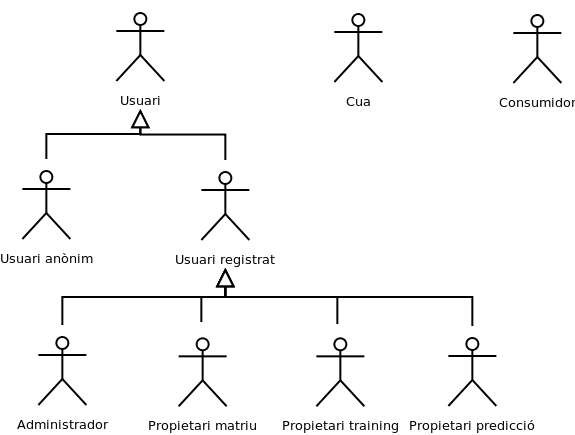
\includegraphics[scale=0.5]{img/specification/Actors.png}
  \caption{Actors}
  \label{specification:actors}
\end{figure}
\begin{itemize}
\item Usuari an\`{o}nim: usuari sense compte al sistema.
\item Usuari registrat: usuari amb compte al sistema.
\begin{itemize}
\item Propietari d'una matriu: usuari que ha creat una matriu.
\item Propietari d'un ''training'': usuari que ha creat un entrenament.
\item Propietari d'una predicci\'{o}: usuair que ha creat una matriu de predicci\'{o}.
\end{itemize}
\item Usuari administrador: usuari amb permissos administratius.
\item Cua: sistema que gestiona les execucions
\item Consumidor: sistema que gestiona les sortides de les execucions.
\item Sistema: sistema que rep les peticions i gestiona les sortides.
\end{itemize}

\section{Casos d'us i fluxos}
En la documentaci\'{o} s'utilitzar\`{a} la seg\�{u}ent estructura per definir els casos d'\'{u}s:\\

\begin{usecase}
\addtitle{Identificador}{Nom cas d'us}
\addfield{Actors:}{Llista de actors}
\addscenario{Curs t\'{i}pic d'esdeveniments:}{
	\item Esdeveniment
	\item Esdeveniment
	\item ...
}
\addscenario{Cursos alternatius:}{
\item Esdeveniment Alternatiu
}
\end{usecase}


\subsection{Crear un usuari}
\begin{usecase}
\addtitle{Usuari001}{Crear un usuari}
\addfield{Actors:}{Anonim}
\addscenario{Curs t\'{i}pic d'esdeveniments:}{
	\item Usuari accedeix al formulari de registraci\'{o}. L'usuari introdueix un nom d'usuari, un correu electr\`{o}nic i una contrasenya per duplicat
	\item El sistema envia al usuari una confirmaci\'{o} via correu electr\'{o}nic amb un enlla� de confirmaci\'{o} i crea un compte no validada.
	\item L'usuari accedeix mitjan�ant l'enlla� de confirmaci\'{o}.
	\item El sistema comprova que \'{e}s un enlla� de confirmaci\'{o} v\`{a}lid d'aquest usuari i activa la compte. L'usuari ja est\'{a} autenticat al sistema com un usuari i ja \'{e}s un usuari del sistema.
}
\addscenario{Cursos alternatius:}{
\item[3] El sistema valida que no existeixi un usuari amb aquesta compte de correu, que el correu sigui v\`{a}lid. Sino es correcte li informa a l'usuari al mateix formulari.
}
\end{usecase}

\subsection{Canviar un usuari de grup}
\begin{usecase}
\addtitle{Usuari002}{Canviar un usuari de grup}
\addfield{Actors:}{Anonim}
\addscenario{Curs t\'{i}pic d'esdeveniments:}{
	\item L'administrador llista tots els usuaris del sistema i selecciona un.
	\item L'administrador veu el formulari de edici\'{o} de permisos.
	\item L'administrador selecciona el nou perm\'{s} i salva el perfil.
	\item El sistema guarda el nou perm\'{i}s
}
\end{usecase}

\subsection{Crear una variable}
\begin{usecase}
\addtitle{Variable001}{Crear una variable}
\addfield{Actors:}{Usuari administrador}
\addscenario{Curs t\'{i}pic d'esdeveniments:}{
	\item L'usuari visualitza el formulari on pot donar un identificador que ha de ser \'{u}nic en el sistema i una descripci\'{o} .
	\item El sistema crear la variable.
}
\end{usecase}

\subsection{Actualitzar una variable}
\begin{usecase}
\addtitle{Variable002}{Actualitzar una variable}
\addfield{Actors:}{Usuari administrador}
\addscenario{Curs t\'{i}pic d'esdeveniments:}{
    \item L'admininistrador seleccion un variable d'un llistat de variables.
    \item El sistema li mostra un formulari d'edici\'{o} on pot veure, les ''season sets'' i els seus components(''seasons'') i pot actualitzar la descripci\'{o}.
    \item L'usuari modifica la descripci\'{o} i salva els canvis.
    \item El sistema guarda les modificacions.
}
\end{usecase}

\subsection{Crear una season set}
\begin{usecase}
\addtitle{Variable003}{Crear una ''season set''}
\addfield{Actors:}{Usuari registrat}
\addscenario{Curs t\'{i}pic d'esdeveniments:}{
	\item L'usuari selecciona una variable d'un llistat de variables.
	\item El sistema li mostra un formulari d'edici\'{o} de la variable amb un enlla� a un formulari de creaci\'{o}.
	\item L'usuari accedeix a un formulari de creaci\'{o} de ''season set''.
	\item El sistema li mostra un formulari de creaci\'{o}.
	\item L'usuari pot donar un nom i seleccionar 0, 1 o 2 fitxers amb el contingut dels ''seasons'', on cada fitxer pot ser configurat com:
	\begin{itemize}
		\item a unic per tot l'any
		\item com estiu
		\item com hivern
		\item com tardor
		\item com estiu
	\end{itemize}	
	\item L'usuari salva els canvis.
	\item El sistema guarda els canvis.
}
\end{usecase}

\subsection{Actualitzar una ''season set''}
\begin{usecase}
\addtitle{Variable004}{Actualitzar una ''season set''}
\addfield{Actors:}{Usuari registrat}
\addscenario{Curs t\'{i}pic d'esdeveniments:}{
    \item L'usuari selecciona una variable d'un llistat de variables.
    \item El sistema li mostra un formulari d'edici\'{o} on pot editar el nom.
    \item L'usuari selecciona una ''season set''.
    \item El sistema li mostra un formulari on pot actualitzar una ''season set''
    \item L'usuari actualiza les dades i guarda els canvis.
    \item El sistema guarda els canvis. 
}
\end{usecase}

\subsection{Esborrar una ''season set''}
\begin{usecase}
\addtitle{Variable005}{Crear una ''season set''}
\addfield{Actors:}{Usuari registrat}
\addscenario{Curs t\'{i}pic d'esdeveniments:}{
    \item L'usuari selecciona una variable d'un llistat de variables per esborrar.
    \item El sistema li mostra un vista de confirmaci\'{o} de la acci\'{o}.
    \item L'usuari confirma la acci\'{o}.
    \item El sistema esborra una ''season set'' i els seus components(''seasons'').
}
\addscenario{Cursos alternatius:}{
\item[3] L'usuari cancela la acci\'{o}.
}
\end{usecase}

\subsection{Afegir una nova ''season'' a una ''season set''}
\begin{usecase}
\addtitle{Variable006}{Afegir una nova ''season'' d'una ''season set''}
\addfield{Actors:}{Usuari registrat}
\addscenario{Curs t\'{i}pic d'esdeveniments:}{
    \item L'usuari selecciona una variable d'un llistat de variables.
    \item El sistema li mostra un formulari de edici\'{o} dels components(''seasons'').
    \item L'usuari pot donar un nom i seleccionar 0, 1 o 2 fitxers amb el contingut dels ''seasons'', on cada fitxer pot ser configurat com:
	\begin{itemize}
		\item a unic per tot l'any
		\item com estiu
		\item com hivern
		\item com tardor
		\item com estiu
	\end{itemize}
	\item L'usuari salva els canvis.
	\item El sistema guarda els canvis.
}
\end{usecase}

\subsection{Esborrar una ''season'' d'una ''season set''}
\begin{usecase}
\addtitle{Variable007}{Esborrar una ''season'' d'una ''season set''}
\addfield{Actors:}{Usuari registrat}
\addscenario{Curs t\'{i}pic d'esdeveniments:}{
    \item L'usuari selecciona una variable d'un llistat de variables.
    \item El sistema li mostra un formulari de edici\'{o} dels components(''seasons'').
	\item L'usuari selecciona una ''season'' per esborrar.
	\item El sistema li demana confirmaci\'{o}.
	\item L'usuari confirma l'acci\'{o}
	\item El sistema esborra el component ''season''
}
\addscenario{Cursos alternatius:}{
\item[5] L'usuari cancela la acci\'{o}.
}
\end{usecase}


\subsection{Crear un matriu des d'un fitxer}
\begin{usecase}
\addtitle{Matriu001}{Crear una matrius des d'un fitxer}
\addfield{Actors:}{Usuari registrat}
\addscenario{Curs t\'{i}pic d'esdeveniments:}{
	\item L'usuari accedeix a un formulari on pot donar nom a la matriu i seleccionar el fitxer en format csv o excel. L'usuari accepta el formulari.
	\item El sistema crear la matriu on:
	\begin{itemize}
	\item La primera fila del fitxer s'associa com una variable Ichnaea. Si la variable es igual al identificador de la variable, automaticament s'assigna a aquesta columna a aquesta variable i a un conjunt de ''seasons''(''season sets'') per defecte.
	\item Cada fila del fitxer, despr\'{e}s de la primera fila:
	\begin{itemize}
		\item La primera columna \'{e}s el identificador de la mostra. Si cont\'{e} un alias d'origen, autom\`{a}ticament s'assigna un origen
		\item Les columnes restants s'assignan com a valors de la mostra
	\end{itemize}
	\item L'usuari visualitza la matriu.
	\end{itemize}
}
\end{usecase}

\subsection{Actualitzar una matriu}
\begin{usecase}
\addtitle{Matriu002}{Actualitzar una matriu}
\addfield{Actors:}{Propietari de la matriu}
\addscenario{Curs t\'{i}pic d'esdeveniments:}{
	\item L'usuari selecciona una matriu per actualitzar.
	\item El sistema li mostra un formulari d'edici\'{o} de la matriu.
	\item L'usuari accedeix a un formulari on pot actualitzar el nom a la matriu i/o seleccionar el fitxer de tipus de fulla de c\`{a}lcul. L'usuari confirma els canvis
	\item El sistema esborra la matriu anterior i torna a crear la matriu on:
	\begin{itemize}
	\item La primera fila del fitxer s'associa com una variable Ichnaea. Si la variable es igual al identificador de la variable, automaticament s'assigna a aquesta columna a aquesta variable i a un conjunt de ''seasons''(''season sets'') per defecte.
	\item Cada fila del fitxer, despr\'{e}s de la primera fila:
	\begin{itemize}
		\item La primera columna \'{e}s el identificador de la mostra. Si cont\'{e} un alias d'origen, autom\`{a}ticament s'assigna un origen
		\item Les columnes restants s'assignan com a valors de la mostra
	\end{itemize}
	\end{itemize}
	\item L'usuari visualitza la matriu.
}
\end{usecase}

\subsection{Clonar una matriu}
\begin{usecase}
\addtitle{Matriu003}{Clonar una matriu}
\addfield{Actors:}{Usuari registrat}
\addscenario{Curs t\'{i}pic d'esdeveniments:}{
	\item L'usuari selecciona una matriu per clonar.
	\item El sistema renderitza un formulari amb un nom suggerit per la matriu.
	\item L'usuari pot canviar el nom i acceptar la clonaci\'{o}.
	\item El sistema clona la matriu i la seva configuraci\'{o} sense copiar ''trainings'' ni prediccions. El propietari de la matriu \'{e}s l'usuari que ha realitzat la clonaci\'{o}. 
	\item L'usuari veu la matriu clonada.
}
\end{usecase}

\subsection{Esborra una matriu}
\begin{usecase}
\addtitle{Matriu004}{Esborrar una matriu}
\addfield{Actors:}{Propietari de la matriu}
\addscenario{Curs t\'{i}pic d'esdeveniments:}{
	\item L'usuari selecciona una matriu del sistema per esborrara.
	\item El sistema demana confirmaci\'{o} per esborrar la matriu.
	\item L'usuari confirma la acci\'{o}.
	\item El sistema clona la matriu i la seva configuraci\'{o} sense copiar trainigs ni prediccions. El propietari de la matriu \'{e}s l'usuari que ha realitzat la clonaci\'{o}.
}
\addscenario{Cursos alternatius:}{
	\item[3] L'usuari cancela la acci\'{o}.
}
\end{usecase}

\subsection{Configurar una columna de la matriu}
\begin{usecase}
\addtitle{Matriu005}{Configurar la columna de una matriu}
\addfield{Actors:}{Usuari propietari de la matriu}
\addscenario{Curs t\'{i}pic d'esdeveniments:}{
	\item L'usuari selecciona una matriu
	\item El sistema mostra una vista per configurar les columnes de una matriu.
	\item L'usuari selecciona una columna i pot:
	\begin{itemize}
		\item donar un nom a la columna
		\item seleccionar una variable i una 'season set' de la variable
	\end{itemize}
	\item L'usuari accepta la configuraci\'{o}
	\item El sistema salva la configuraci\'{o} de la columna
}
\end{usecase}


\subsection{Configurar el ''sample'' d'una matriu}
\begin{usecase}
\addtitle{Matriu 004}{Configurar la data del ''sample'' de una matriu}
\addfield{Actors:}{Usuari propietari de una matriu}
\addscenario{Curs t\'{i}pic d'esdeveniments:}{
	\item L'usuari selecciona un matriu.
	\item El sistema mostra una vista per configurar les mostres(''samples'') de la matriu.
	\item L'usuari selecciona una ''sample'' i pot:
	\begin{itemize}
	\item donar una data 
	\item donar una nom a la mostra
	\item donar un origen de la mostra
	\end{itemize}
	\item L'usuari accepta la configuraci\'{o}.
	\item El sistema guarda la configuraci\'{o} del ''sample''.
}
\end{usecase}

\subsection{Llistar ''trainings'' del sistema}
\begin{usecase}
\addtitle{Training001}{Llistar ''trainings''}
\addfield{Actors:}{Usuari administrador}
\addscenario{Curs t\'{i}pic d'esdeveniments:}{
	\item L'usuari accedeix a la vista del llistat de ''trainings'' del sistema.
	\item El sistema llista els trainings amb les dades b\`{a}siques: matriu entrenada, estat del training, descripci\'{o} del training, creador, data de creaci\'{o}.
}
\end{usecase}

\subsection{Llistar els meus ''trainings''}
\begin{usecase}
\addtitle{Training002}{Llistar els meus trainings}
\addfield{Actors:}{Usuari registrat}
\addscenario{Curs t\'{i}pic d'esdeveniments:}{
	\item L'usuari accedeix a la vista del llistat de ''trainings'' que ha creat.
	\item El sistema llista els trainings que ha creat amb dades b\`{a}siques: matriu entrenada, estat del training, descripci\'{o} del training, data de creaci\'{o}.
}
\end{usecase}

\subsection{Llistar ''trainings'' entrenables}
\begin{usecase}
\addtitle{Training003}{Llistar ''trainings'' entrenables}
\addfield{Actors:}{Usuari registrat}
\addscenario{Curs t\'{i}pic d'esdeveniments:}{
	\item L'usuari accedeix a la vista del llistat de trainings entrenables.
	\item El sistema llista els ''trainings'' amb un estat finalitzat i sense errors amb dades b\`{a}siques: matriu entrenada, estat del training, creador, descripci\'{o} del training, data de creaci\'{o}.
}
\end{usecase}

\subsection{Crear un ''training''}
\begin{usecase}
\addtitle{Training004}{Crear un ''training''}
\addfield{Actors:}{Usuari registrat}
\addscenario{Curs t\'{i}pic d'esdeveniments:}{
	\item L'usuari selecciona una matriu per entrenar
	\item El sistema li mostra un formulari per crear trainings
	\item L'usuari pot donar un nom, una descripci\'{o}, seleccionar un origen i quines columnes vol entrenar. Confirma les dades.
	\item El sistema guarda el training i envia al sistema de cues les dades. El sistema evalua si ha pogut enviar el training al sistema de cues en cas que el servei estigui caigut. 
	\item L'usuari veu el training creat.
}
\end{usecase}

\subsection{Reenviar un training al sistema de cues}
\begin{usecase}
\addtitle{Training005}{Reenviar un training}
\addfield{Actors:}{Usuari propietari d'un ''training''}
\addscenario{Curs t\'{i}pic d'esdeveniments:}{
    \item L'usuari selecciona un training que ha tingut problemes de enviament.
    \item El sistema renderitza una vista de visualitzaci\'{o} del training.
    \item L'usuari pot consultar quin possible error ha passat i pot confirmar el reenviament
    \item El sistema actulitza les dades i reenvia les dades al sistema de cues.
}
\end{usecase}

\subsection{Visualitzar un training}
\begin{usecase}
\addtitle{Training006}{Visualitzar un training}
\addfield{Actors:}{Usuari registrat}
\addscenario{Curs t\'{i}pic d'esdeveniments:}{
    \item L'usuari selecciona d'un llistat un training.
    \item El sistema renderitza una vista de visualitzaci\'{o} del training amb el nom, descripci\'{o}, data de creaci\'{o} i  errors o resultats segons el cas.
}
\end{usecase}

\subsection{Esborrar un ''training''}
\begin{usecase}
\addtitle{Training007}{Esborrar un ''training''}
\addfield{Actors:}{Usuari superadministrador, usuari propietari d'un ''training''}
\addscenario{Curs t\'{i}pic d'esdeveniments:}{
	\item L'usuari selecciona un ''training'' per esborrar
	\item El sistema demana confirmaci\'{o} per esborrar el training.
	\item L'usuari confirma l'acci\'{o}
	\item El sistema esborra el ''trainings'' i totes les prediccions que s'han fet a partir d'aquest ''training''.
}
\end{usecase}

\subsection{Descarregar els resultats d'un ''training''}
\begin{usecase}
\addtitle{Training008}{Descarregar els resultats d'un ''training''}
\addfield{Actors:}{Usuari registrat}
\addscenario{Curs t\'{i}pic d'esdeveniments:}{
    \item L'usuari selecciona un training finalitzat
    \item El sistema visualitza un enlla� amb la possibilitat de descarregar el fitxer resultats d'un ''training''
    \item L'usuari accedeix a la descarrega.
    \item El sistema envia a l'usuari els resultats.
}
\end{usecase}

\subsection{Actualitzar l'estat d'un ''training''}
\begin{usecase}
\addtitle{Training009}{Actualitzar l'estat d'un ''training''}
\addfield{Actors:}{Cua}
\addscenario{Curs t\'{i}pic d'esdeveniments:}{
    \item La cua avisa al consumidor que ha finalitzat un ''training'' i li envia unes dades al consumidor
    \item El consumidor rep les dades i li envia al sistema
    \item El sistema les guarda i actulitza l'estat del ''training''
}
\end{usecase}

\subsection{Llistar prediccions del sistema}
\begin{usecase}
\addtitle{Prediction001}{Llistar prediccions del sistema}
\addfield{Actors:}{Usuari administrador}
\addscenario{Curs t\'{i}pic d'esdeveniments:}{
	\item L'usuari accedeix a la vista del llistat de prediccions
	\item El sistema llista totes les prediccions amb dades b\`{a}siques.
}
\end{usecase}

\subsection{Llistar les meves prediccions}
\begin{usecase}
\addtitle{Prediction002}{Llistar les meves prediccions}
\addfield{Actors:}{Usuari registrats}
\addscenario{Curs t\'{i}pic d'esdeveniments:}{
	\item L'usuari accedeix a la vista del llistat de prediccions creades per ell.
	\item EL sistema llista totes les prediccions creades per l'usuari amb dades b\`{a}siques.
}
\end{usecase}

\subsection{Esborrar una predicci\'{o}}
\begin{usecase}
\addtitle{Prediction003}{Esborrar una predicci\'{o}}
\addfield{Actors:}{Usuari registrats}
\addscenario{Curs t\'{i}pic d'esdeveniments:}{
	\item L'usuari selecciona una predicci\'{o} per esborrar.
	\item El sistema li demana confirmaci\'{o} per esborrar la predicci\'{o}.
	\item L'usuari confirma la acci\'{o}.
	\item El sistema esborra la predicci\'{o}.
}
\addscenario{Cursos alternatius:}{
	\item[3] L'usuari cancela la acci\'{o}.
}
\end{usecase}

\subsection{Crear una matriu de predicci\'{o} desde un fitxer}
\begin{usecase}
\addtitle{Prediction004}{Crear una matriu de predicci\'{o} desde un fitxer}
\addfield{Actors:}{Usuari registrats}
\addscenario{Curs t\'{i}pic d'esdeveniments:}{
	\item L'usuari selecciona un entrenament(''training'') per crear una predicci\'{o}.
	\item El sistema li mostra un formulari de creaci\'{o} de prediccions.
	\item L'usuari accedeix a un formulari on pot donar nom a la matriu de predicci\'{o} i seleccionar una fulla de c\`{a}lcul. L'usuari accepta el formulari.
	\item El sistema crear la matriu on:
	\begin{itemize}
	\item Cada fila del fitxer, despr\'{e}s de la primera fila:
	\begin{itemize}
		\item La primera columna \'{e}s el identificador de la mostra. Si cont\'{e} un alias d'origen, autom\`{a}ticament s'assigna un origen
		\item Les columnes restants s'assignan com a valors de la mostra
	\end{itemize}
	\item L'usuari visualitza la matriu.
	\end{itemize}
}
\end{usecase}

\subsection{Actualitzar una matriu de predicci\'{o} desde un fitxer}
\begin{usecase}
\addtitle{Prediction005}{Actualitzar una matriu de predicci\'{o} desde un fitxer}
\addfield{Actors:}{Usuari propietari de la predicci\'{o}}
\addscenario{Curs t\'{i}pic d'esdeveniments:}{
    \item L'usuari seleccion un entrenament
    \item El sistema li mostra un formulari d'edici\'{o} de prediccions.
    \item L'usuari pot actualitzar el nom de la predicci\'{o} i seleccionar una fulla de c\'{a}lcul i guardar els canvis.
    \item El sistema esborra la matrius de predicci\'{o}, actualitza les dades i crea la matriu on:
    	\begin{itemize}
	\item Cada fila de la fulla de calcul, despr\'{e}s de la primera fila:
	\begin{itemize}
		\item La primera columna \'{e}s el identificador de la mostra. Si cont\'{e} un alias d'origen, autom\`{a}ticament s'assigna un origen
		\item Les columnes restants s'assignan com a valors de la mostra
	\end{itemize}
	\item L'usuari visualitza la matriu.
	\end{itemize}
}
\end{usecase}

\subsection{Configurar un ''sample'' d'una matriu de predicci\'{o}}
\begin{usecase}
\addtitle{Prediction 006}{Configurar un ''sample'' d'una matriu de predicci\'{o}}
\addfield{Actors:}{Usuari propietari de la predicci\'{o}}
\addscenario{Curs t\'{i}pic d'esdeveniments:}{
	\item L'usuari selecciona una predicci\'{o} i una mostra.
	\item El sistema mostra una vista de edici\'{o} de la matriu.
	\item L'usuari pot donar un data, un nom i un origen a la mostra i guardar els canvis.
	\item El sistema guarda les dades.
}
\end{usecase}

\subsection{Enviar una predicci\'{o} al sistema de cues}
\begin{usecase}
\addtitle{Prediction007}{Enviar una predicci\'{o} al sistema de cues}
\addfield{Actors:}{Usuari propietari de la predicci\'{o}}
\addscenario{Curs t\'{i}pic d'esdeveniments:}{
    \item L'usuari selecciona una predicci\'{o}.
    \item El sistema li mostra un formulari per enviar la matriu de predicci\'{o} al sistema de cues.
    \item L'usuari confirma la acci\'{o}.
    \item El sitema prepara les dades per enviar i li dona al sistema de cues.
}
\end{usecase}

\subsection{Veure una predicci\'{o}}
\begin{usecase}
\addtitle{Prediction008}{Veure una predicci\'{o}}
\addfield{Actors:}{Usuari registrat}
\addscenario{Curs t\'{i}pic d'esdeveniments:}{
	\item L'usuari selecciona una predicci\'{o}.
	\item El sistema li mostra les dades b\`{a}siques de la predicci\'{o} i la matriu de predicci\'{o}.
}
\end{usecase}

\subsection{Veure els resultats d'una predicci\'{o}}
\begin{usecase}
\addtitle{Prediction009}{Veure els resultats d'una predicci\'{o}}
\addfield{Actors:}{Usuari registrat}
\addscenario{Curs t\'{i}pic d'esdeveniments:}{
	\item L'usuari selecciona els resultats d'una predicci\'{o}.
	\item El sistema li mostra les diferents sortides de la execuci\'{o}.
}
\end{usecase}

\subsection{Actualitzar l'estat d'una predicci\'{o}}
\begin{usecase}
\addtitle{Prediction010}{Actualitzar l'estat d'una predicci\'{o}}
\addfield{Actors:}{Cua, Consumidor}
\addscenario{Curs t\'{i}pic d'esdeveniments:}{
    \item La cua avisa al consumidor que ha finalitzat una predicci\'{o} i li envia les dades al consumidor
    \item El consumidor rep les dades i li envia al sistema
    \item El sistema les guarda i actulitza l'estat de la predicci\'{o}.
}
\end{usecase}

\section{Model de dades}
En el seg\�{u}ent diagrama UML est\`{a} implementat el modelatge de dades.
\begin{sidewaysfigure}[h]
  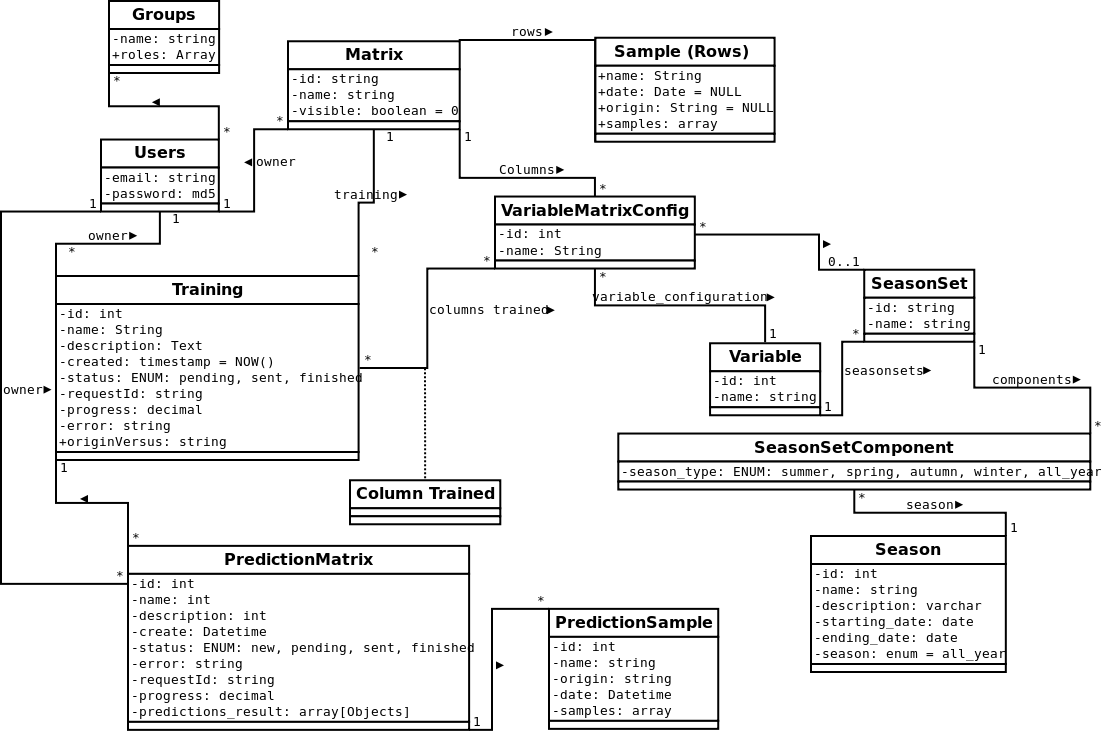
\includegraphics[scale=0.5]{img/specification/ModelClass.png}
  \caption{Model de dades}
  \label{specification:datamodel}
\end{sidewaysfigure}